%%%%%%%%%%%%%%%%%%%%%%%%%%%%%%%%%%%%%%%%%%%%%%%%%%%%%%%%
% Este é um documento que servirá de modelo para
% os relatórios feitos na disciplina Laboratório de Circuitos Lógicos
% 2020-2
%%%%%%%%%%%%%%%%%%%%%%%%%%%%%%%%%%%%%%%%%%%%%%%%%%%%%%%%%

%%%%%%%%%%%%%%%%%%%%%%%%%%%%%%%%%%%%%%%%%%%%%%%%%%%%%%%%%
% Use os diferentes diretórios para colocar os relatórios de cada experimento, deste modo vc consegue manter um histórico e todo material organizado em apenas um local.
% Lembre-se de mudar o Main Document no Menu!!!

\documentclass[12pt]{article}

\usepackage{sbc-template}
\usepackage[brazil]{babel}
\usepackage{graphicx}
\usepackage{url}
\usepackage{float}
\usepackage{listings}
\usepackage{color}
%\usepackage{todonotes}
\usepackage{algorithmic}
\usepackage{algorithm}
\usepackage{hyperref}
\hypersetup{
    colorlinks=true,
    linkcolor=black,
    filecolor=magenta,      
    urlcolor=blue,
    citecolor=black
    }
     
\sloppy
\raggedbottom

\title{Experimento 6\\ 
Circuitos Combinacionais: Codificador e Decodificador}

\author{Grupo B2 - Turma T2\\   
        Allan Victor Almeida Faria, 261010546\\
        Caio César Gonçalves Ribeiro,  211038217\\
        Danilo Alves Ribeiro,  242003754\\
}


\address{Dep. Ciência da Computação -- Universidade de Brasília (UnB)\\
  CIC0231 - Laboratório de Circuitos Lógicos\\
  \today
  \email{allanvictor.almeida@gmail.com, caiocesar20032003@gmail.com, daniloalvesjob@gmail.com}
}

\begin{document} 
\maketitle

\selectlanguage{american}
 \begin{abstract}
This report describes the design, minimization, simulation, and FPGA implementation of a decimal-to-Gray encoder and a Gray-to-decimal decoder. The Boolean functions were derived from the Gray code table and simplified with Karnaugh maps, using the don't-care conditions created by invalid input combinations. The encoder was reduced to four sums of inputs, with seventeen literals in total, and the decoder to ten product terms, with thirty-two literals, six of which do not depend on the most significant bit. Functional and temporal simulations in Quartus-II reproduced the expected truth tables, and the encoder/decoder pair synthesized on the DE2-70 kit converted each decimal digit selected on the switches to the corresponding LED. The results confirm the equivalence between the minimized expressions and the physical implementation, and show that the single-bit adjacency of the Gray code allows adjacent minterms to be grouped, reducing the decoder hardware.
 \end{abstract}
\selectlanguage{brazil}     
 \begin{resumo} 
Este relatório descreve o projeto, a minimização, a simulação e a implementação em FPGA de um codificador de decimal para código de Gray e de um decodificador de Gray para decimal. As funções booleanas foram obtidas da tabela do código de Gray e simplificadas por mapas de Karnaugh, aproveitando as condições optativas geradas pelas entradas inválidas. O codificador ficou com quatro somas de entradas, dezessete literais no total, e o decodificador com dez produtos, trinta e dois literais, sendo que seis saídas não dependem do bit mais significativo. As simulações funcional e temporal no Quartus-II reproduziram as tabelas-verdade previstas, e o par codificador/decodificador sintetizado no kit DE2-70 converteu cada dígito decimal selecionado nas chaves ao LED correspondente. Os resultados confirmam a equivalência entre as expressões minimizadas e a implementação física e mostram que a adjacência de um único bit do código de Gray permite agrupar mintermos vizinhos, reduzindo o hardware do decodificador.
 \end{resumo}


\section{Introdução}
\label{sec:Introducao}

Em sistemas digitais, o processamento interno de informações é realizado predominantemente no sistema binário, devido à simplicidade e à confiabilidade dos circuitos eletrônicos de dois níveis de tensão. Na interação com o usuário e com equipamentos de entrada/saída, porém, a representação utilizada é a decimal. Para converter informações entre esses domínios, utilizam-se circuitos combinacionais denominados codificadores e decodificadores \cite{wakerly90}.

Um \textit{codificador} recebe um conjunto de linhas de entrada, em que apenas uma é ativada por vez, e produz nas saídas o código binário correspondente. O \textit{decodificador} faz o inverso: recebe um código binário e ativa a única saída associada àquela combinação. Entre os códigos existentes, o código de Gray destaca-se por alterar apenas um bit entre símbolos consecutivos. No projeto desses circuitos, as condições optativas (\textit{don't care}) permitem simplificar bastante as expressões booleanas.

Neste experimento, foram projetados, minimizados e sintetizados em FPGA um codificador de decimal para Gray e um decodificador de Gray para decimal, com diagramas no Quartus-II, simulações funcional e temporal e validação no kit DE2-70.

\subsection{Objetivos}
\label{sec:Objetivos}

Os objetivos do experimento são:
\begin{itemize}
    \item Projetar um codificador de decimal para Gray e um decodificador de Gray para decimal, aplicando minimização booleana com condições optativas;
    \item Elaborar os diagramas esquemáticos no Quartus-II e realizar as simulações funcional e temporal;
    \item Sintetizar e validar os circuitos no kit de desenvolvimento FPGA DE2-70.
\end{itemize}

\subsection{Materiais} 
\label{sec:Materiais}

Foram utilizados:
\begin{itemize}
    \item Software Quartus-II versão 13.0 SP1;
    \item Kit de desenvolvimento em FPGA DE2-70 Intel;
    \item Cabo de programação USB-Blaster.
\end{itemize}

\section{Procedimentos e Resultados}
\label{sec:Procedimentos}

Antes de descrever os circuitos, registra-se que a filmagem do funcionamento no kit não foi realizada, o que é uma falha de organização do grupo. A execução do experimento, contudo, é comprovada pelo desempenho nas etapas de Pré-Projeto e de Pós-Experimento, em que os circuitos foram apresentados e testados no kit e receberam a pontuação correspondente. Falta, portanto, apenas o registro em vídeo. A Tabela~\ref{tab:gray} apresenta o código adotado.

\begin{table}[H]
    \centering
    \caption{Código de Gray para os dígitos decimais (Tabela I do roteiro).}
    \label{tab:gray}
    \begin{tabular}{|c|c|c|c|c|}
        \hline
        Decimal & $A$ & $B$ & $C$ & $D$ \\
        \hline
        0 & 0 & 0 & 0 & 0 \\
        \hline
        1 & 0 & 0 & 0 & 1 \\
        \hline
        2 & 0 & 0 & 1 & 1 \\
        \hline
        3 & 0 & 0 & 1 & 0 \\
        \hline
        4 & 0 & 1 & 1 & 0 \\
        \hline
        5 & 0 & 1 & 1 & 1 \\
        \hline
        6 & 0 & 1 & 0 & 1 \\
        \hline
        7 & 0 & 1 & 0 & 0 \\
        \hline
        8 & 1 & 1 & 0 & 0 \\
        \hline
        9 & 1 & 1 & 0 & 1 \\
        \hline
    \end{tabular}
\end{table}

\subsection{Codificador decimal para Gray}
\label{sec:Encoder}

O codificador recebe as dez chaves do kit, uma para cada dígito, e gera em $A$, $B$, $C$ e $D$ o código de Gray correspondente. Como apenas uma chave deve estar acionada, as combinações com duas ou mais chaves são inválidas e foram tratadas como condições optativas; o mesmo vale para o dígito 0, cujo código é $0000$ e não depende das chaves.

Para cada saída, assinalaram-se com $1$ os dígitos cujo código tem aquele bit igual a $1$ e com $X$ as combinações inválidas. A minimização por mapas de Karnaugh forneceu:

\[
\begin{array}{rcl}
    A & = & X_8 + X_9 \\[2pt]
    B & = & X_4 + X_5 + X_6 + X_7 + X_8 + X_9 \\[2pt]
    C & = & X_2 + X_3 + X_4 + X_5 \\[2pt]
    D & = & X_1 + X_2 + X_5 + X_6 + X_9
\end{array}
\]

\noindent em que $X_i$ é a chave do dígito $i$. A forma canônica teria dez mintermos de dez literais; a minimização reduziu o circuito a quatro portas OU, com dezessete literais e nenhum inversor. O diagrama esquemático é mostrado na Figura~\ref{fig:encoder}.

\begin{figure}[H]
    \centering
    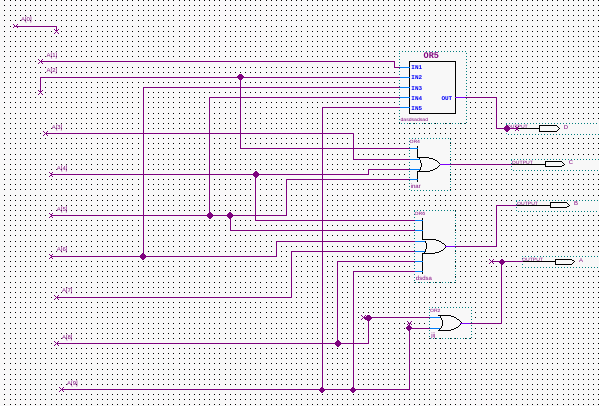
\includegraphics[width=.9\textwidth]{encoder.png}
    \caption{Diagrama esquemático do codificador decimal para Gray no Quartus-II.}
    \label{fig:encoder}
\end{figure}

Na Figura~\ref{fig:encoder}, cada porta OU tem um número de entradas igual ao número de termos da respectiva soma, e as chaves ligadas diretamente às portas correspondem aos literais das equações.

\subsubsection{Simulações do codificador}

As simulações funcional e temporal foram feitas no editor de formas de onda do Quartus-II. O estímulo percorre todas as combinações das dez chaves; nos intervalos em que apenas uma chave está ativa, as saídas assumem exatamente os valores da Tabela~\ref{tab:gray}. A simulação temporal mostrou que os atrasos das portas OU não alteram os níveis após o transitório. As capturas são mostradas nas Figuras~\ref{fig:sim-encoder-funcional} e~\ref{fig:sim-encoder-temporal}; nelas, as dez linhas decimais aparecem como $A_0$ a $A_9$.

\begin{figure}[H]
    \centering
    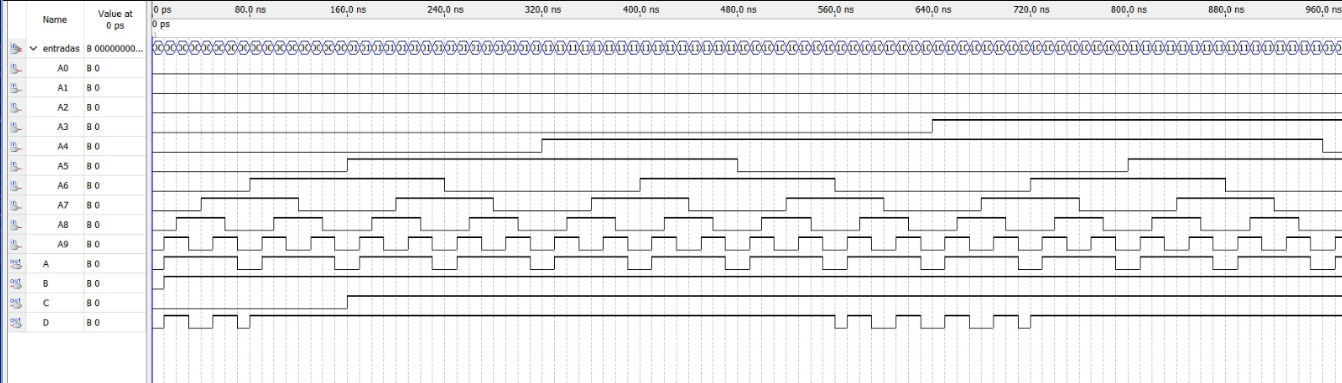
\includegraphics[width=\textwidth]{simfuncionalencoder.png}
    \caption{Simulação funcional do codificador: entradas $A_0$ a $A_9$ e saídas $A$, $B$, $C$ e $D$.}
    \label{fig:sim-encoder-funcional}
\end{figure}

\begin{figure}[H]
    \centering
    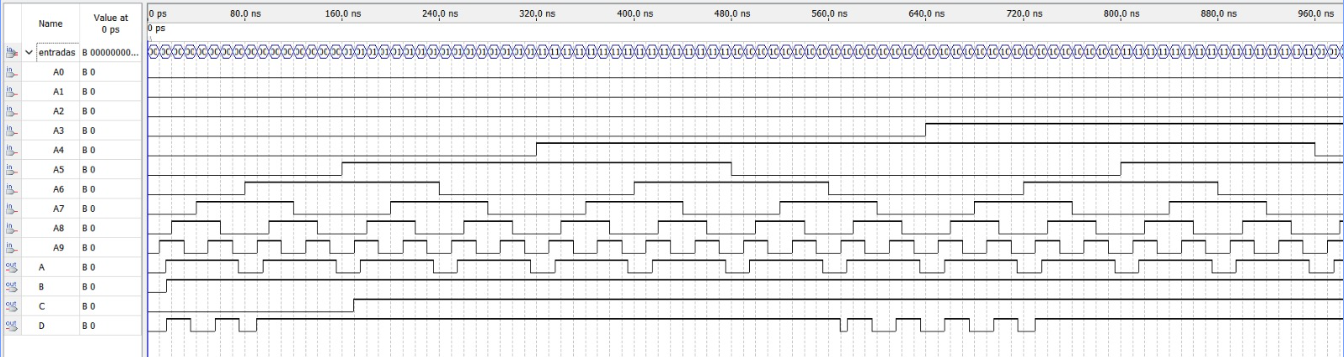
\includegraphics[width=\textwidth]{simtemporalencoder.png}
    \caption{Simulação temporal do codificador, com os atrasos de propagação das portas OU.}
    \label{fig:sim-encoder-temporal}
\end{figure}

\subsection{Decodificador Gray para decimal}
\label{sec:Decoder}

O decodificador recebe $A$, $B$, $C$ e $D$ e ativa uma única saída $S_i$, correspondente ao dígito $i$. Cada saída é $1$ apenas quando a entrada é igual ao código daquele dígito; as seis combinações de $1010$ a $1111$ não representam dígitos e foram tratadas como condições optativas. A minimização resultou em:

\[
\begin{array}{rclcrcl}
    S_0 & = & \bar{B}\bar{C}\bar{D} & \qquad & S_5 & = & B\,C\,D \\[2pt]
    S_1 & = & \bar{B}\bar{C}D & \qquad & S_6 & = & \bar{A}B\bar{C}D \\[2pt]
    S_2 & = & \bar{B}C\,D & \qquad & S_7 & = & \bar{A}B\bar{C}\bar{D} \\[2pt]
    S_3 & = & \bar{B}C\bar{D} & \qquad & S_8 & = & A\bar{C}\bar{D} \\[2pt]
    S_4 & = & B\,C\bar{D} & \qquad & S_9 & = & A\,D
\end{array}
\]

A Tabela~\ref{tab:decoder} apresenta a tabela-verdade completa, com as dezesseis combinações de entrada; nas linhas inválidas as saídas são marcadas com ``--''.

\begin{table}[H]
    \centering
    \small
    \caption{Tabela-verdade completa do decodificador Gray para decimal.}
    \label{tab:decoder}
    \begin{tabular}{|c|c|c|c||c|c|c|c|c|c|c|c|c|c|}
        \hline
        $A$ & $B$ & $C$ & $D$ & $S_0$ & $S_1$ & $S_2$ & $S_3$ & $S_4$ & $S_5$ & $S_6$ & $S_7$ & $S_8$ & $S_9$ \\
        \hline
        0 & 0 & 0 & 0 & 1 & 0 & 0 & 0 & 0 & 0 & 0 & 0 & 0 & 0 \\
        \hline
        0 & 0 & 0 & 1 & 0 & 1 & 0 & 0 & 0 & 0 & 0 & 0 & 0 & 0 \\
        \hline
        0 & 0 & 1 & 1 & 0 & 0 & 1 & 0 & 0 & 0 & 0 & 0 & 0 & 0 \\
        \hline
        0 & 0 & 1 & 0 & 0 & 0 & 0 & 1 & 0 & 0 & 0 & 0 & 0 & 0 \\
        \hline
        0 & 1 & 1 & 0 & 0 & 0 & 0 & 0 & 1 & 0 & 0 & 0 & 0 & 0 \\
        \hline
        0 & 1 & 1 & 1 & 0 & 0 & 0 & 0 & 0 & 1 & 0 & 0 & 0 & 0 \\
        \hline
        0 & 1 & 0 & 1 & 0 & 0 & 0 & 0 & 0 & 0 & 1 & 0 & 0 & 0 \\
        \hline
        0 & 1 & 0 & 0 & 0 & 0 & 0 & 0 & 0 & 0 & 0 & 1 & 0 & 0 \\
        \hline
        1 & 1 & 0 & 0 & 0 & 0 & 0 & 0 & 0 & 0 & 0 & 0 & 1 & 0 \\
        \hline
        1 & 1 & 0 & 1 & 0 & 0 & 0 & 0 & 0 & 0 & 0 & 0 & 0 & 1 \\
        \hline
        1 & 0 & 1 & 0 & -- & -- & -- & -- & -- & -- & -- & -- & -- & -- \\
        \hline
        1 & 0 & 1 & 1 & -- & -- & -- & -- & -- & -- & -- & -- & -- & -- \\
        \hline
        1 & 0 & 0 & 0 & -- & -- & -- & -- & -- & -- & -- & -- & -- & -- \\
        \hline
        1 & 0 & 0 & 1 & -- & -- & -- & -- & -- & -- & -- & -- & -- & -- \\
        \hline
        1 & 1 & 1 & 0 & -- & -- & -- & -- & -- & -- & -- & -- & -- & -- \\
        \hline
        1 & 1 & 1 & 1 & -- & -- & -- & -- & -- & -- & -- & -- & -- & -- \\
        \hline
    \end{tabular}
\end{table}

O diagrama lógico foi dividido em duas folhas apenas por organização. A Figura~\ref{fig:decoder1} traz as negações de $D$ e $C$ e as portas de $S_0$ a $S_5$; a Figura~\ref{fig:decoder2}, as negações de $B$ e $A$ e as portas de $S_6$ a $S_9$.

\begin{figure}[H]
    \centering
    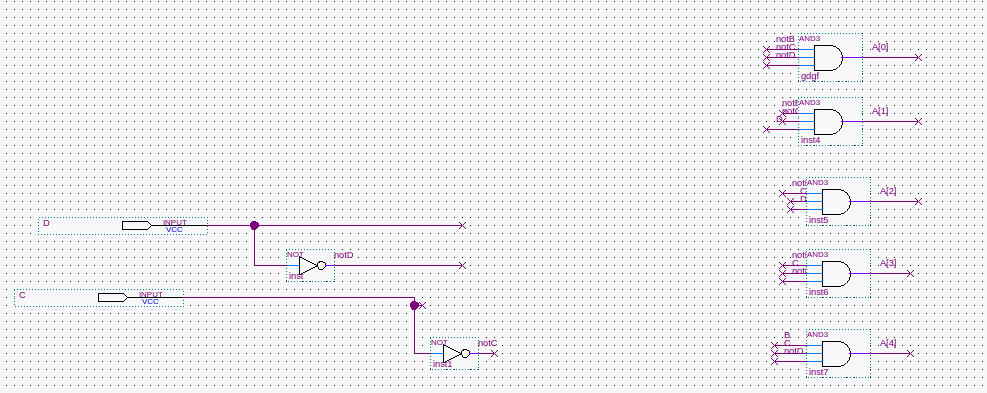
\includegraphics[width=\textwidth]{decoderprimeiraparte.png}
    \caption{Primeira parte do decodificador no Quartus-II: portas de $S_0$ a $S_5$.}
    \label{fig:decoder1}
\end{figure}

\begin{figure}[H]
    \centering
    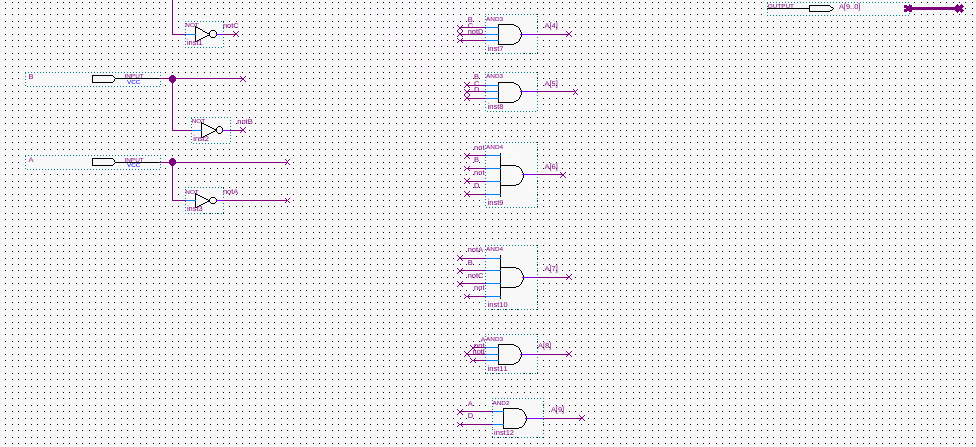
\includegraphics[width=\textwidth]{decoderparte2.png}
    \caption{Segunda parte do decodificador no Quartus-II: portas de $S_6$ a $S_9$.}
    \label{fig:decoder2}
\end{figure}

\subsubsection{Simulações do decodificador}

A simulação funcional usou como estímulo um contador de quatro bits em código de Gray, conforme sugerido no roteiro, que percorre os dezesseis códigos. Nos dez válidos, apenas $S_i$ fica em nível alto, na ordem dos dígitos; nos seis inválidos, nenhuma saída é ativada, o que aparece na forma de onda como um intervalo sem saída ativa entre $S_7$ e $S_8$. A simulação temporal confirmou que os atrasos das portas E e das negações não afetam o resultado após o transitório. As capturas são mostradas nas Figuras~\ref{fig:sim-decoder-funcional} e~\ref{fig:sim-decoder-temporal}, nas quais as dez linhas decimais aparecem como $A_0$ a $A_9$.

\begin{figure}[H]
    \centering
    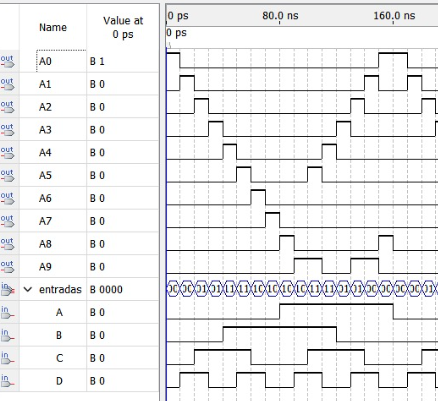
\includegraphics[width=.8\textwidth]{simfuncionaldecoder.png}
    \caption{Simulação funcional do decodificador: entradas $A$, $B$, $C$ e $D$ em código de Gray e saídas $A_0$ a $A_9$.}
    \label{fig:sim-decoder-funcional}
\end{figure}

\begin{figure}[H]
    \centering
    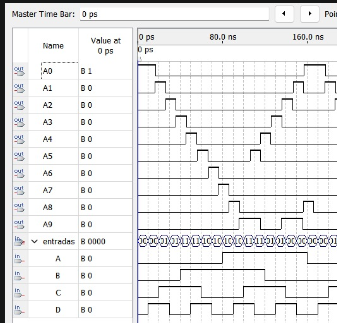
\includegraphics[width=.6\textwidth]{simtemporaldecoder.png}
    \caption{Simulação temporal do decodificador, com os atrasos das portas E e das negações.}
    \label{fig:sim-decoder-temporal}
\end{figure}

\subsubsection{Vantagem do código de Gray na minimização do decodificador}
\label{sec:vantagem-gray}

No decodificador BCD, as saídas de 0 a 7 exigem, cada uma, um produto de quatro literais, porque dígitos consecutivos diferem em vários bits e seus mintermos não são adjacentes no mapa de Karnaugh. No código de Gray, dois símbolos consecutivos diferem em apenas um bit, de modo que os mintermos vizinhos são sempre adjacentes e podem ser agrupados. Por isso, as saídas $S_0$ a $S_5$ dispensaram o bit $A$ e ficaram com três literais, e $S_9$ reduziu-se a $A\,D$. No total, o decodificador de Gray ficou com trinta e dois literais, contra trinta e oito do BCD equivalente.

\subsection{Pós-Experimento: integração no kit FPGA}
\label{sec:PosExperimento}

Na etapa final, o codificador e o decodificador foram ligados em cascata, conforme a Figura 4 do roteiro: as chaves selecionam o dígito decimal, o codificador gera o código de Gray e o decodificador reconstrói o dígito, indicado por um LED. O esquema integrado é mostrado na Figura~\ref{fig:integrado}.

\begin{figure}[H]
    \centering
    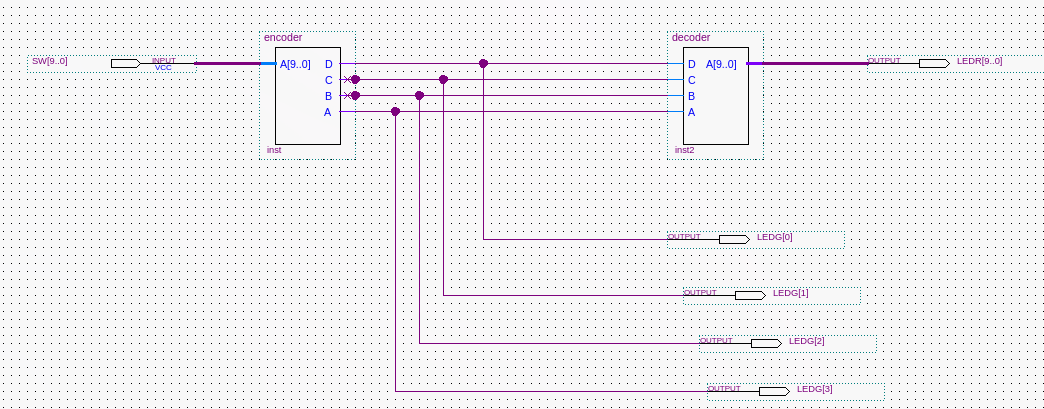
\includegraphics[width=.85\textwidth]{circuitofigura.png}
    \caption{Circuito integrado: as chaves \texttt{SW[9..0]} alimentam o codificador, cujas saídas também vão para \texttt{LEDG[3..0]}, e o decodificador ativa uma das saídas \texttt{LEDR[9..0]}.}
    \label{fig:integrado}
\end{figure}

Na Figura~\ref{fig:integrado}, os bits do código de Gray são levados ao decodificador e, ao mesmo tempo, aos LEDs verdes, o que permite conferir visualmente o código gerado; a saída do decodificador vai para os LEDs vermelhos. O resultado esperado para cada dígito está na Tabela~\ref{tab:integrado}.

\begin{table}[H]
    \centering
    \caption{Resultado esperado da integração codificador/decodificador.}
    \label{tab:integrado}
    \begin{tabular}{|c|c|c|c|}
        \hline
        Dígito & $A\,B\,C\,D$ (\texttt{LEDG}) & LED aceso (\texttt{LEDR}) & Saída ativa \\
        \hline
        0 & 0000 & \texttt{LEDR[0]} & $S_0$ \\
        \hline
        1 & 0001 & \texttt{LEDR[1]} & $S_1$ \\
        \hline
        2 & 0011 & \texttt{LEDR[2]} & $S_2$ \\
        \hline
        3 & 0010 & \texttt{LEDR[3]} & $S_3$ \\
        \hline
        4 & 0110 & \texttt{LEDR[4]} & $S_4$ \\
        \hline
        5 & 0111 & \texttt{LEDR[5]} & $S_5$ \\
        \hline
        6 & 0101 & \texttt{LEDR[6]} & $S_6$ \\
        \hline
        7 & 0100 & \texttt{LEDR[7]} & $S_7$ \\
        \hline
        8 & 1100 & \texttt{LEDR[8]} & $S_8$ \\
        \hline
        9 & 1101 & \texttt{LEDR[9]} & $S_9$ \\
        \hline
    \end{tabular}
\end{table}

No kit, o circuito foi sintetizado e testado com uma chave acionada por vez. Para todos os dez dígitos, o LED correspondente acendeu, os demais permaneceram apagados e os LEDs verdes exibiram o código da Tabela~\ref{tab:gray}. A condição de nenhuma chave acionada também leva a $0000$ e ao LED do dígito 0, o que é coerente com o projeto. Combinações com duas ou mais chaves não têm significado definido, pois foram tratadas como condições optativas.

\section{Conclusões}
\label{sec:Conclusao}

O experimento cumpriu os objetivos propostos. Os circuitos foram projetados, minimizados e desenhados no Quartus-II, e as simulações funcional e temporal reproduziram as tabelas-verdade previstas. No kit DE2-70, cada dígito selecionado nas chaves acendeu o LED correspondente, confirmando o funcionamento do conjunto codificador/decodificador.

A principal lição do experimento foi a vantagem do código de Gray sobre o BCD no decodificador: como símbolos consecutivos diferem em apenas um bit, os mintermos vizinhos são adjacentes e podem ser agrupados, o que gera expressões menores. Ficou claro também que as condições optativas são o que torna essa simplificação possível e que a escolha do código faz parte do projeto do circuito.

\bibliographystyle{sbc}
\bibliography{relatorio}  %Aqui é a definição do arquivo .bib a ser usado pelas referências


\newpage 
% Colocar aqui apenas as respostas dos itens da Auto-Avaliação
\section*{Auto-Avaliação}

\begin{enumerate}
    \item c
    \item c
    \item c
    \item b
    \item c
    \item e
    \item b
    \item f
\end{enumerate}


\end{document}
